
\documentclass[oneside,9pt]{book} % Dimensione font leggermente ridotta
\usepackage{amsmath, amsthm, amssymb, amsfonts}
\usepackage{thmtools}
\usepackage{graphicx}
\usepackage{setspace}
\usepackage{geometry}
\usepackage{float}
\usepackage[pdfencoding=auto]{hyperref}
\usepackage[utf8]{inputenc}
\usepackage[italian]{babel}
\usepackage{framed}
\usepackage[dvipsnames]{xcolor}
\usepackage{environ}
\usepackage{tcolorbox}
\tcbuselibrary{theorems,skins,breakable}
\usepackage{bookmark} % Risolve warning sui segnalibri
\usepackage{enumitem} % Per controllo spaziatura elenchi
\usepackage{parskip}
\usepackage[utf8]{inputenc}  % per LaTeX2e
\usepackage[T1]{fontenc}
\usepackage[italian]{babel}
\tcbuselibrary{theorems,skins,breakable}
\usepackage{float}
\usepackage[section]{placeins} 

\setstretch{1.15} % Spaziatura leggermente ridotta per compattezza
\geometry{
    textheight=9in,
    textwidth=5.5in,
    top=1in,
    headheight=12pt,
    headsep=25pt,
    footskip=30pt
}
%  --- Variabili personalizzate ---
\def\notetitle{Analisi I}
\def\noteauthor{
    \textbf{Gianmarco Davini} \\
    Appunti di Analisi I}
\def\notedate{Anno Accademico 2025/2026}


% Comandi matematici (solo quelli non ridondanti)
\newcommand{\sube}{\subseteq}
\newcommand{\sub}{\subset}
\newcommand{\notsub}{\not\subset}
\newcommand{\rarr}{\rightarrow}
\newcommand{\N}{\mathbb{N}}
\newcommand{\Z}{\mathbb{Z}}
\newcommand{\Q}{\mathbb{Q}}
\newcommand{\R}{\mathbb{R}}

% Configurazione elenchi (spaziatura uniforme)
\setlist[itemize]{topsep=4pt, partopsep=2pt, itemsep=2pt, parsep=2pt}
\setlist[enumerate]{topsep=4pt, partopsep=2pt, itemsep=2pt, parsep=2pt}
% The theorem system and user-defined commands
% Theorem System
% The following boxes are provided:
%   Definition:     \defn 
%   Theorem:        \thm 
%   Lemma:          \lem
%   Corollary:      \cor
%   Proposition:    \prop   
%   Claim:          \clm
%   Fact:           \fact
%   Proof:          \pf
%   Example:        \ex
%   Remark:         \rmk (sentence), \rmkb (block)
% Suffix
%   r:              Allow Theorem/Definition to be referenced, e.g. thmr
%   p:              Add a short proof block for Lemma, Corollary, Proposition or Claim, e.g. lemp
%                   For theorems, use \pf for proof blocks

% Definition
\newtcbtheorem[number within=section]{mydefinition}{Definizione}
{
    enhanced,
    frame hidden,
    titlerule=0mm,
    toptitle=1mm,
    bottomtitle=1mm,
    fonttitle=\bfseries\large,
    coltitle=black,
    colbacktitle=green!20!white,
    colback=green!10!white,
}{defn}

\NewDocumentCommand{\defn}{m+m}{
    \begin{mydefinition}{#1}{}
        #2
    \end{mydefinition}
}

\NewDocumentCommand{\defnr}{mm+m}{
    \begin{mydefinition}{#1}{#2}
        #3
    \end{mydefinition}
}

% Theorem
\newtcbtheorem[use counter from=mydefinition]{mytheorem}{Teorema}
{
    enhanced,
    frame hidden,
    titlerule=0mm,
    toptitle=1mm,
    bottomtitle=1mm,
    fonttitle=\bfseries\large,
    coltitle=black,
    colbacktitle=cyan!20!white,
    colback=cyan!10!white,
}{thm}

\NewDocumentCommand{\thm}{m+m}{
    \begin{mytheorem}{#1}{}
        #2
    \end{mytheorem}
}

\NewDocumentCommand{\thmr}{mm+m}{
    \begin{mytheorem}{#1}{#2}
        #3
    \end{mytheorem}
}

% Lemma
\newtcbtheorem[use counter from=mydefinition]{mylemma}{Lemma}
{
    enhanced,
    frame hidden,
    titlerule=0mm,
    toptitle=1mm,
    bottomtitle=1mm,
    fonttitle=\bfseries\large,
    coltitle=black,
    colbacktitle=violet!20!white,
    colback=violet!10!white,
}{lem}

\NewDocumentCommand{\lem}{m+m}{
    \begin{mylemma}{#1}{}
        #2
    \end{mylemma}
}

\newenvironment{lempf}{
	{\noindent{\it \textbf{Proof for Lemma}}}
	\tcolorbox[blanker,breakable,left=5mm,parbox=false,
    before upper={\parindent15pt},
    after skip=10pt,
	borderline west={1mm}{0pt}{violet!20!white}]
}{
    \textcolor{violet!20!white}{\hbox{}\nobreak\hfill$\blacksquare$} 
    \endtcolorbox
}

\NewDocumentCommand{\lemp}{m+m+m}{
    \begin{mylemma}{#1}{}
        #2
    \end{mylemma}

    \begin{lempf}
        #3
    \end{lempf}
}

% Corollary
\newtcbtheorem[use counter from=mydefinition]{mycorollary}{Corollario}
{
    enhanced,
    frame hidden,
    titlerule=0mm,
    toptitle=1mm,
    bottomtitle=1mm,
    fonttitle=\bfseries\large,
    coltitle=black,
    colbacktitle=orange!20!white,
    colback=orange!10!white,
}{cor}

\NewDocumentCommand{\cor}{+m}{
    \begin{mycorollary}{}{}
        #1
    \end{mycorollary}
}

\newenvironment{corpf}{
	{\noindent{\it \textbf{Proof for Corollary.}}}
	\tcolorbox[blanker,breakable,left=5mm,parbox=false,
    before upper={\parindent15pt},
    after skip=10pt,
	borderline west={1mm}{0pt}{orange!20!white}]
}{
    \textcolor{orange!20!white}{\hbox{}\nobreak\hfill$\blacksquare$} 
    \endtcolorbox
}

\NewDocumentCommand{\corp}{m+m+m}{
    \begin{mycorollary}{}{}
        #1
    \end{mycorollary}

    \begin{corpf}
        #2
    \end{corpf}
}

% Proposition
\newtcbtheorem[use counter from=mydefinition]{myproposition}{Proposizione}
{
    enhanced,
    frame hidden,
    titlerule=0mm,
    toptitle=1mm,
    bottomtitle=1mm,
    fonttitle=\bfseries\large,
    coltitle=black,
    colbacktitle=yellow!30!white,
    colback=yellow!20!white,
}{prop}

\NewDocumentCommand{\prop}{+m}{
    \begin{myproposition}{}{}
        #1
    \end{myproposition}
}

\newenvironment{proppf}{
	{\noindent{\it \textbf{Proof for Proposition.}}}
	\tcolorbox[blanker,breakable,left=5mm,parbox=false,
    before upper={\parindent15pt},
    after skip=10pt,
	borderline west={1mm}{0pt}{yellow!30!white}]
}{
    \textcolor{yellow!30!white}{\hbox{}\nobreak\hfill$\blacksquare$} 
    \endtcolorbox
}

\NewDocumentCommand{\propp}{+m+m}{
    \begin{myproposition}{}{}
        #1
    \end{myproposition}

    \begin{proppf}
        #2
    \end{proppf}
}

% Claim
\newtcbtheorem[use counter from=mydefinition]{myclaim}{Affermazione}
{
    enhanced,
    frame hidden,
    titlerule=0mm,
    toptitle=1mm,
    bottomtitle=1mm,
    fonttitle=\bfseries\large,
    coltitle=black,
    colbacktitle=pink!30!white,
    colback=pink!20!white,
}{clm}


\NewDocumentCommand{\clm}{m+m}{
    \begin{myclaim*}{#1}{}
        #2
    \end{myclaim*}
}

\newenvironment{clmpf}{
	{\noindent{\it \textbf{Proof for Claim.}}}
	\tcolorbox[blanker,breakable,left=5mm,parbox=false,
    before upper={\parindent15pt},
    after skip=10pt,
	borderline west={1mm}{0pt}{pink!30!white}]
}{
    \textcolor{pink!30!white}{\hbox{}\nobreak\hfill$\blacksquare$} 
    \endtcolorbox
}

\NewDocumentCommand{\clmp}{m+m+m}{
    \begin{myclaim*}{#1}{}
        #2
    \end{myclaim*}

    \begin{clmpf}
        #3
    \end{clmpf}
}

% Fact
\newtcbtheorem[use counter from=mydefinition]{myfact}{Fatto}
{
    enhanced,
    frame hidden,
    titlerule=0mm,
    toptitle=1mm,
    bottomtitle=1mm,
    fonttitle=\bfseries\large,
    coltitle=black,
    colbacktitle=purple!20!white,
    colback=purple!10!white,
}{fact}

\NewDocumentCommand{\fact}{+m}{
    \begin{myfact}{}{}
        #1
    \end{myfact}
}


% Proof
\NewDocumentCommand{\pf}{+m}{
    \begin{proof}
        [\noindent\textbf{Dimostrazione.}]
        #1
    \end{proof}
}

% Example
\newenvironment{example}{
    \par
    \vspace{5pt}
    \noindent\textbf{Esempio.}
    \begin{tcolorbox}[
        blanker, breakable, left=5mm, parbox=false,
        before upper={\parindent15pt},
        after skip=10pt,
        borderline west={1mm}{0pt}{cyan!10!white}]
}{
    \end{tcolorbox}
    \vspace{5pt}
}

\NewDocumentCommand{\ex}{+m}{
    \begin{example}
        #1
    \end{example}
}

% Remark
\NewDocumentCommand{\rmk}{+m}{
    {\it \color{black!50!white}#1}
}

\newenvironment{remark}{
    \par
    \vspace{5pt}
    \noindent\textbf{Osservazione.}
    \begin{tcolorbox}[
        blanker, breakable, left=5mm, parbox=false,
        before upper={\parindent15pt},
        after skip=10pt,
        borderline west={1mm}{0pt}{cyan!10!white}]
}{
    \end{tcolorbox}
    \vspace{5pt}
}

\NewDocumentCommand{\rmkb}{+m}{
    \begin{remark}
        #1
    \end{remark}
}


\newcommand{\lcm}{\operatorname{lcm}}



% --- Inizio documento ---
\begin{document}
\title{\textbf{\LARGE{\notetitle} \vspace*{10\baselineskip}}}
\author{\noteauthor}
\date{\notedate}
\maketitle
\newpage
\setcounter{tocdepth}{3}
\tableofcontents
\newpage
% =================================================================
\chapter{Funzioni}
% =============================================================================

\section{Funzioni astratte}

\defn{Funzione}{
Siano $A, B \ne \emptyset$. Si chiama \textbf{funzione} $f: A \rarr B$ una legge che associa \textbf{ad ogni elemento di $A$ uno ed un solo elemento di $B$}.
Si può anche scrivere:
\[
f: x \in A \mapsto y = f(x) \in B
\]
dove $y$ è l'\textbf{immagine} di $x$ mediante $f$.
}

\begin{itemize}
    \item $A$ si dice \textbf{dominio} di $f$ (insieme di esistenza)
    \item $B$ si dice \textbf{codominio} di $f$
    \item L'insieme
    \[
    f(A) = \{\, y \in B \mid \exists x \in A : y = f(x) \,\}
    \]
    si chiama \textbf{immagine} di $A$
    \item Sia $y \in B$, con $f^{-1}(y)$ indichiamo il seguente insieme:
    \[
    f^{-1}(y) = \{\, x \in A \mid f(x) = y \,\}
    \]
    Questo insieme può avere, a seconda dei casi, nessuno ($\emptyset$), uno o più elementi.
    \item L'insieme
    \[
    G(f) = \{\, (x, f(x)) \mid x \in A \,\}
    \]
    si chiama \textbf{grafico} di $f$
\end{itemize}

\subsection{Restrizione}

\defn{Restrizione}{
Sia $f: A \rarr B$ con $A, B \ne \emptyset$.
Sia $E \subseteq A$, $E \ne \emptyset$.
La funzione
\[
g: E \rarr B, \quad g(x) = f(x) \text{ per ogni } x \in E
\]
si chiama \textbf{restrizione di $f$ su $E$} e si indica con $f|_E$.
}

\subsection{Funzioni composte}
Siano $A, B, C \ne \emptyset$ e siano $f: A \to B$ e $g: B \to C$.
Allora si definisce la \textbf{funzione composta} $g \circ f: A \to C$ mediante
\[
(g \circ f)(x) = g(f(x)), \quad \forall x \in A
\]
dove $(g \circ f)(x)$ è l'immagine di $x$ tramite la composizione di $f$ e $g$.

\ex{
\[
f(x) = x + 1, \quad f: \mathbb{R} \to \mathbb{R} \\
g(x) = x^3, \quad g: \mathbb{R} \to \mathbb{R}
\]
Allora:
\[
(g \circ f)(x) = g(f(x)) = (x + 1)^3, \quad x \in \mathbb{R} \\
(f \circ g)(x) = f(g(x)) = x^3 + 1, \quad x \in \mathbb{R}
\]
Questi esempi mostrano chiaramente che la composizione \textbf{non è commutativa}.
}

\subsection{Funzioni suriettive}
Una funzione $f: A \to B$ si dice \textbf{suriettiva} se l'immagine coincide con il codominio, cioè:
\[
\forall b \in B, \ \exists a \in A \mid f(a) = b
\]
In una funzione suriettiva la controimmagine di ogni elemento del codominio \textbf{non può essere vuota}.

\subsection{Funzioni iniettive}
Una funzione $f: A \to B$ si dice \textbf{iniettiva} se elementi distinti del dominio hanno immagini distinte, cioè:
\[
\forall x_1, x_2 \in A, \ f(x_1) = f(x_2) \implies x_1 = x_2
\]
oppure equivalentemente:
\[
x_1, x_2 \in A, \ x_1 \ne x_2 \implies f(x_1) \ne f(x_2)
\]
In una funzione iniettiva la controimmagine di ogni elemento del codominio può avere \textbf{al massimo un elemento}.

\subsection{Funzioni biettive}
Una funzione $f: A \to B$ si dice \textbf{biettiva} se è sia iniettiva che suriettiva.
\begin{itemize}
    \item Esiste quindi una \textbf{corrispondenza biunivoca} tra gli elementi del dominio e del codominio.
    \item La controimmagine di ogni elemento del codominio possiede \textbf{esattamente un elemento}.
    \item In simboli:
    \[
    f(A) = B, \quad x_1 \ne x_2 \implies f(x_1) \ne f(x_2)
    \]
\end{itemize}

\subsection{Identità}
\defn{Funzione Identità}{
Sia $A \ne \emptyset$.
La \textbf{funzione identità} su $A$, indicata con $i_A$, è definita da:
\[
i_A: x \in A \mapsto x \in A
\]
}

Se la funzione è biettiva si definisce la funzione inversa
\[
f^{-1}: B \to A, \quad y \in B \mapsto x = f^{-1}(y)
\]
Avendo $f: A \to B$ e $f^{-1}: B \to A$ possiamo comporle per ottenere le funzioni identità di $A$ e identità di $B$ ($i_A$ e $i_B$):
\begin{itemize}
    \item $f \circ f^{-1}: y \in B \mapsto y \in B = i_B$
    \item $f^{-1} \circ f: x \in A \mapsto x \in A = i_A$
\end{itemize}

Una funzione biettiva è anche \textbf{invertibile}, cioè esiste $f^{-1}: B \to A$ tale che:
\[
f^{-1}(f(x)) = x, \quad \forall x \in A
\]

L'esistenza della funzione inversa è ciò che ci permette di risolvere le disequazioni, prendiamo ad esempio la disequazione $x^2 \leq 8$:
\begin{itemize}
    \item La funzione potenza $f(x) = x^2$ non è invertibile su tutto $\mathbb{R}$, ma diventa invertibile se ristretta al dominio $\mathbb{R}^+_0$ (numeri reali non negativi). La sua inversa è la funzione radice quadrata $f^{-1}(y) = \sqrt{y}$, definita per $y \geq 0$.

    \item Utilizzando la funzione inversa, possiamo risolvere la disequazione $x^2 \leq 8$ applicando la radice quadrata a entrambi i membri. Tuttavia, dobbiamo considerare che $x^2$ è definita per tutti gli $x \in \mathbb{R}$, quindi dobbiamo separare i casi in base al segno di $x$:
    \begin{itemize}
        \item Se $x \geq 0$, allora $x = \sqrt{x^2} \leq \sqrt{8} = 2\sqrt{2}$.
        \item Se $x \leq 0$, allora $x = -\sqrt{x^2} \geq -\sqrt{8} = -2\sqrt{2}$.
    \end{itemize}

    \item Combinando i due casi, otteniamo la soluzione finale:
    \[
    -2\sqrt{2} \leq x \leq 2\sqrt{2}.
    \]
    Questo significa che tutti i valori di $x$ compresi tra $-2\sqrt{2}$ e $2\sqrt{2}$ soddisfano la disequazione $x^2 \leq 8$.
  \end{itemize}

\section{Funzioni Numeriche}
\subsection{Proprietà delle funzioni numeriche}
\subsubsection{Grafico della Funzione}

\defn{Grafico}{
Sia $f : A \subseteq \mathbb{R} \to \mathbb{R}$, con $A \neq \emptyset$.
Si chiama \emph{grafico} di $f$ l'insieme
\[
G(f) = \{(x, f(x)) \mid x \in A\} \subseteq \mathbb{R}^2.
\]
}

Nel piano cartesiano non esiste una relazione d'ordine.
Ad ogni funzione corrisponde un grafico.

\begin{figure}[h]
    \centering
    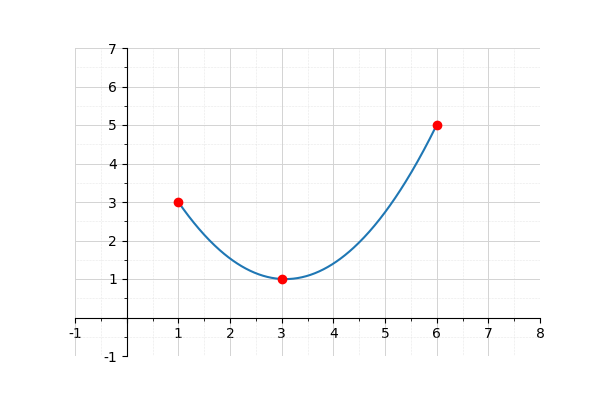
\includegraphics[width=0.7\textwidth]{./img/grafico.png} % sostituire con il file corretto
    \caption{Grafico della funzione}
    \label{fig:grafico_della_funzione}
  \end{figure}
  
Dal grafico di una funzione possiamo ricavare informazioni come il dominio e il codominio anche senza conoscere la legge precisa:
\[
A = [1, 6], \quad f(A) = B = [1, 5].
\]

Dal grafico possiamo capire anche se la funzione è iniettiva.

\subsubsection{Funzione Inversa}

Una funzione è invertibile se e solo se, fissato un valore $y$, esiste una sola $x$ tale che $f(x) = y$.

Se la funzione è invertibile, il grafico della sua inversa è
\[
G(f^{-1}) = \{(y, f^{-1}(y)) \mid y \in f(A)\}.
\]

\begin{figure}[h]
    \centering
    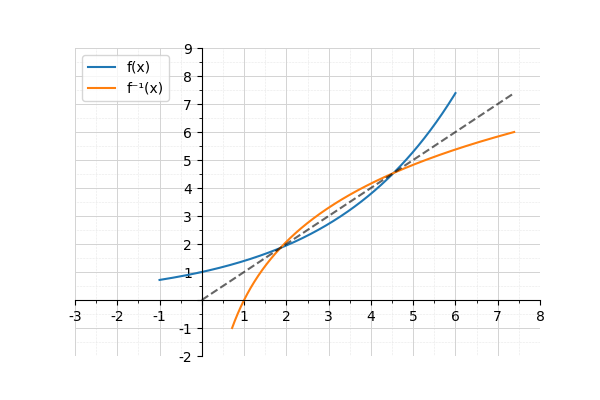
\includegraphics[width=0.7\textwidth]{./img/funzione_inversa.png} % sostituire con il file corretto
    \caption{Grafico della funzione inversa}
    \label{fig:funzione_inversa}
\end{figure}

\subsection{Funzioni Pari e Dispari}

\defn{Proprietà di simmetria}{
  Sia $f: \mathbb{R} \to \mathbb{R}$.  
  La funzione $f$ si dice \emph{pari} se
  \[
    f(-x) = f(x), \quad \forall x \in \mathbb{R},
  \]
  cioè se ha simmetria rispetto all'asse $y$.  

  La funzione $f$ si dice \emph{dispari} se
  \[
    f(-x) = -f(x), \quad \forall x \in \mathbb{R}.
  \]

  La funzione $f$ si dice \emph{periodica} di periodo $t \in \mathbb{R}$ se
  \[
    f(x) = f(x+t), \quad \forall x \in \mathbb{R}.
  \]
}

\begin{figure}[h]
    \centering
    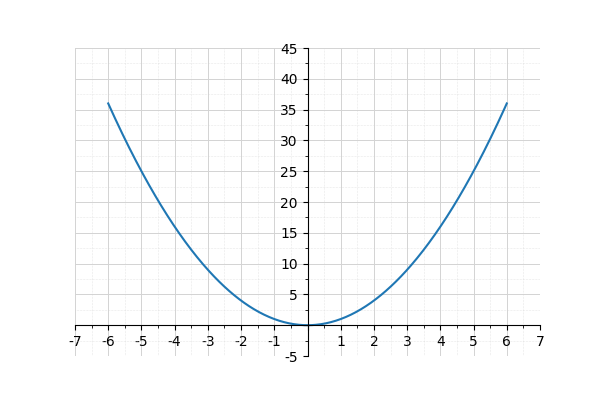
\includegraphics[width=0.7\textwidth]{./img/funzione_pari.png}
    \caption{Esempio di funzione pari}
    \label{fig:funzione_pari}
\end{figure}

\begin{figure}[h]
    \centering
    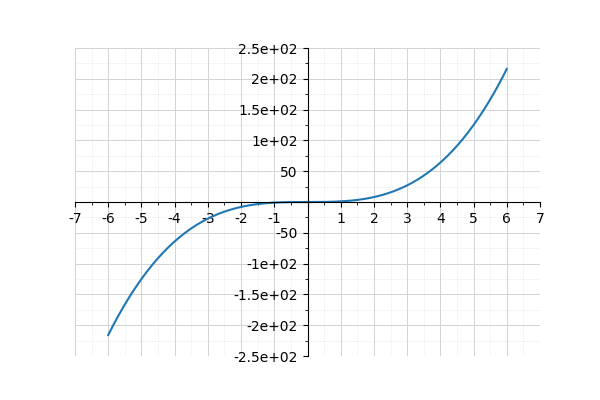
\includegraphics[width=0.7\textwidth]{./img/funzione_dispari.png}
    \caption{Esempio di funzione dispari}
    \label{fig:funzione_dispari}
\end{figure}

\begin{figure}[h]
    \centering
    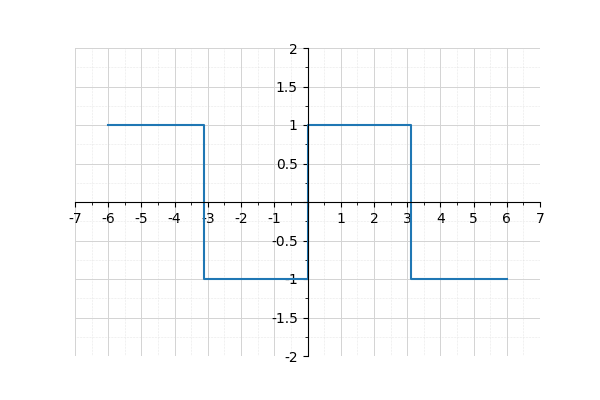
\includegraphics[width=0.7\textwidth]{./img/funzione_periodica.png}
    \caption{Esempio di funzione periodica}
    \label{fig:funzione_periodica}
\end{figure}

\subsection{Funzioni Limitate}

\defn{Funzione superiormente limitata}{
  Sia $f: A \subseteq \mathbb{R} \to \mathbb{R}$ con $A \neq \emptyset$.  
  La funzione $f$ si dice \emph{superiormente limitata} se $f(A)$ è superiormente limitata, cioè se
  \[
    \exists K \in \mathbb{R} \text{ tale che } f(x) \leq K, \quad \forall x \in A.
  \]
}

\defn{Funzione inferiormente limitata}{
  La funzione $f$ si dice \emph{inferiormente limitata} se $f(A)$ è inferiormente limitata, cioè se
  \[
    \exists c \in \mathbb{R} \text{ tale che } c \leq f(x), \quad \forall x \in A.
  \]
}

\defn{Funzione limitata}{
  La funzione $f$ si dice \emph{limitata} se è sia inferiormente che superiormente limitata, cioè se
  \[
    \exists c, K \in \mathbb{R} \text{ tali che } c \leq f(x) \leq K, \quad \forall x \in A.
  \]
}

\defn{Estremo superiore}{
  Si definisce \emph{estremo superiore} di $f(A)$ e si indica con $\sup f(A)$.
}

\defn{Estremo inferiore}{
  Si definisce \emph{estremo inferiore} di $f(A)$ e si indica con $\inf f(A)$.
}

\subsection{Massimo e Minimo}

\defn{Massimo}{
  Sia $f: A \subseteq \mathbb{R} \to \mathbb{R}$ con $A \neq \emptyset$.  
  Se $f(A)$ ha un massimo $M$, diremo che $f$ ha un massimo e scriveremo
  \[
    M = \max f(A).
  \]
  Essendo $M \in f(A)$, esiste $x_M \in A$ tale che $f(x_M) = M$, che si chiama \emph{punto di massimo}. Il punto di massimo non è necessariamente unico.
}

\begin{figure}[h]
    \centering
    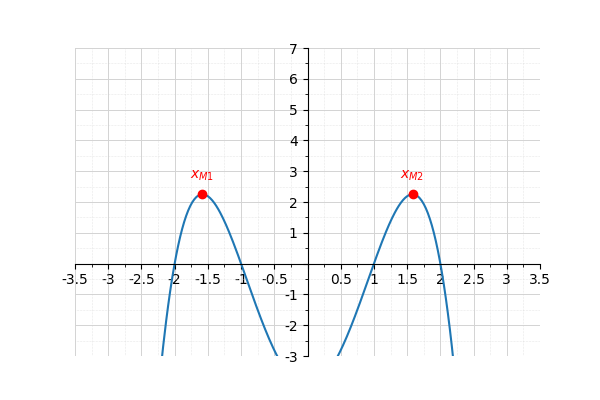
\includegraphics[width=0.7\textwidth]{./img/massimi_della_funzione.png}
    \caption{Esempio di funzione con due punti di massimo}
    \label{fig:punto_di_massimo}
\end{figure}

\defn{Minimo}{
  Se $f(A)$ ha un minimo $m$, diremo che $f$ ha un minimo e i punti $x_m \in A$ tali che $f(x_m) = m$ si chiamano \emph{punti di minimo}.
}

\subsection{Funzioni Monotone}

\defn{Monotona crescente}{
  Sia $f: A \subseteq \mathbb{R} \to \mathbb{R}$ con $A \neq \emptyset$.  
  La funzione $f$ si dice \emph{monotona crescente} se
  \[
    x_1 < x_2, \ x_1, x_2 \in A \implies f(x_1) \leq f(x_2),
  \]
  e \emph{strettamente monotona crescente} se
  \[
    x_1 < x_2 \implies f(x_1) < f(x_2).
  \]
}

\begin{figure}[h]
    \centering
    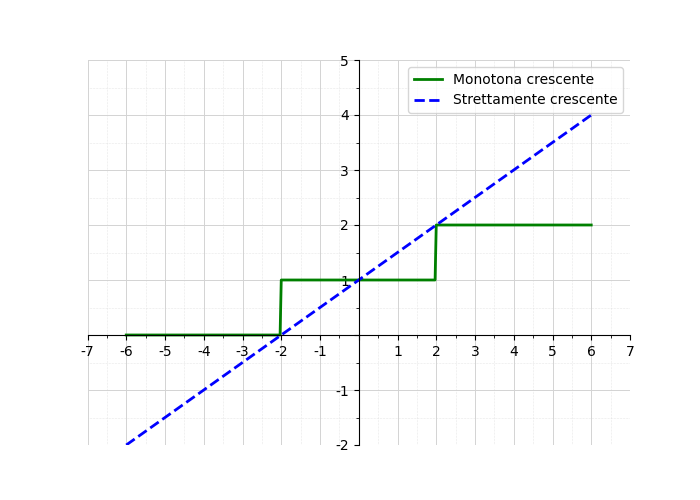
\includegraphics[width=0.7\textwidth]{./img/monotone_crescenti.png}
    \caption{Esempio di funzioni crescenti}
    \label{fig:funzione_crescente}
\end{figure}

\defn{Monotona decrescente}{
  La funzione $f$ si dice \emph{monotona decrescente} se
  \[
    x_1 < x_2 \implies f(x_1) \geq f(x_2),
  \]
  e \emph{strettamente monotona decrescente} se
  \[
    x_1 < x_2 \implies f(x_1) > f(x_2).
  \]
}

\begin{figure}[h]
    \centering
    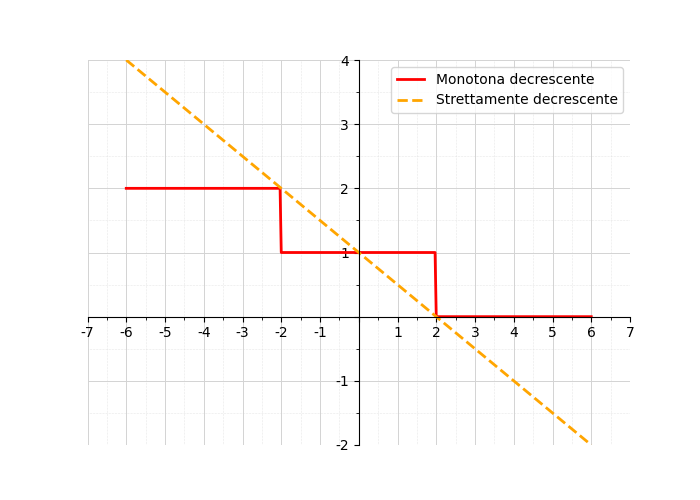
\includegraphics[width=0.7\textwidth]{./img/monotone_decrescenti.png}
    \caption{Esempio di funzioni decrescenti}
    \label{fig:funzione_decrescente}
\end{figure}

Inoltre valgono le seguenti proprietà:
\begin{itemize}
  \item Una funzione strettamente monotona è iniettiva.
  \item Se $f$ è invertibile e monotona, anche $f^{-1}$ è monotona della stessa tipologia.
\end{itemize}

\section{Funzioni Elementari}
\subsection{Funzioni lineari (o affini)}

Sia 
\[
f(x) = a x + b, \quad a, b \in \mathbb{R}, \quad a \neq 0.
\]

\begin{figure}[h]
    \centering
    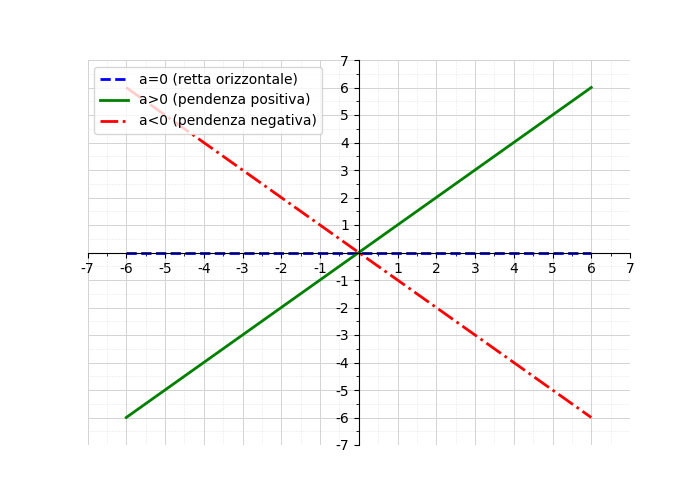
\includegraphics[width=0.7\textwidth]{./img/lineari_combinato.png}
    \caption{Grafico della funzione lineare}
    \label{fig:funzione_lineare}
\end{figure}

Proprietà della funzione lineare:
\begin{itemize}
    \item Se $a > 0$, la funzione è crescente.
    \item Se $a < 0$, la funzione è decrescente.
    \item Se $f(x) = x$ o $f(x) = -x$, la funzione coincide con una bisettrice.
\end{itemize}

\subsection{Funzione valore assoluto}

Sia
\[
|x| = 
\begin{cases} 
x, & \text{se } x \ge 0, \\
-x, & \text{se } x < 0,
\end{cases}
\quad x \in \mathbb{R}, \quad |x| : \mathbb{R} \to [0, +\infty).
\]

\begin{figure}[h]
    \centering
    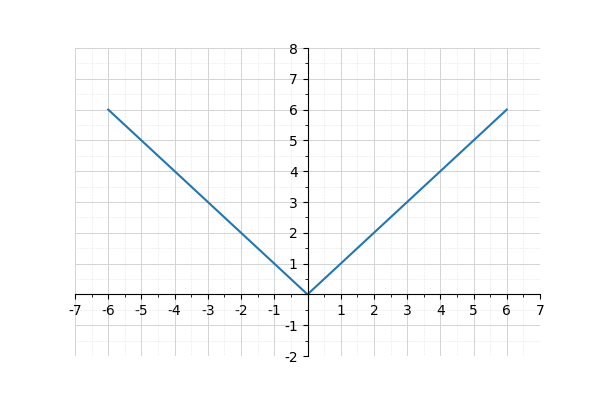
\includegraphics[width=0.7\textwidth]{./img/funzione_valore_assoluto.png}
    \caption{Grafico della funzione valore assoluto}
    \label{fig:funzione_valore_assoluto}
\end{figure}


  

Proprietà della funzione valore assoluto:
\begin{enumerate}
    \item $|x| \ge 0$ per ogni $x \in \mathbb{R}$.
    \item $|x| = 0 \iff x = 0$.
    \item $|-x| = |x|$, quindi la funzione è pari.
    \item $|x_1 \cdot x_2| = |x_1| \cdot |x_2|$.
    \item $|x| \le a \iff -a \le x \le a$.
    \item $|x| \ge a \iff x \le -a \ \text{o} \ x \ge a$.
    \item Per ogni $x_1, x_2 \in \mathbb{R}$ vale la \emph{disuguaglianza triangolare}:
    \[
    |x_1 + x_2| \le |x_1| + |x_2|.
    \]
    Dimostrazione:
    \begin{align*}
    -|x_1| \le x_1 \le |x_1|, \quad -|x_2| \le x_2 \le |x_2| \\
    \implies -(|x_1| + |x_2|) \le x_1 + x_2 \le |x_1| + |x_2| \\
    \implies |x_1 + x_2| \le |x_1| + |x_2|.
    \end{align*}
  \end{enumerate}
\subsection{Funzione potenza (con esponente in $\mathbb{N}$)}
$f: x \in \mathbb{R} \mapsto x^n \in$
\begin{itemize}
\item $[0, +\infty)$ per $n$ pari
\item $\mathbb{R}$ per $n$ dispari
\end{itemize}
$f(x) = x^n$

\subsubsection{Caso $n$ pari}
\begin{figure}[H]
    \centering
    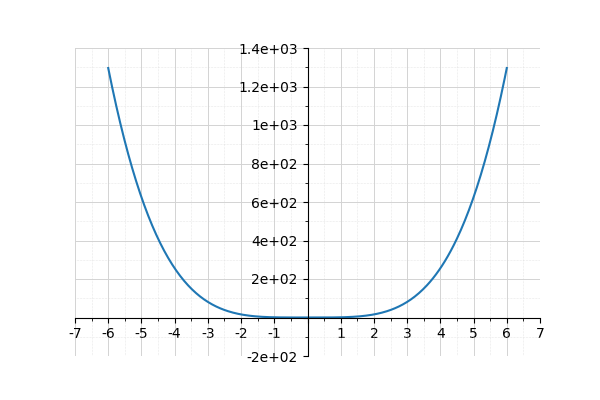
\includegraphics[width=0.7\textwidth]{./img/esponente_pari.png}
    \caption{Grafico della funzione per $n$ pari}
    \label{fig:esponente_pari}
\end{figure}
\FloatBarrier
\begin{itemize}
\item La funzione è pari
\item $x^n \geq 0 \quad \forall x \in \mathbb{R}$, $x^n=0 \iff x=0$
\item Non è globalmente monotona:
    \begin{itemize}
    \item $x^n$ strettamente crescente per $x\geq 0$
    \item $x^n$ strettamente decrescente per $x\leq 0$
    \end{itemize}
\item $\sup_{x \in \mathbb{R}} x^n = +\infty$
\item $\inf_{x \in \mathbb{R}} x^n = \min_{x \in \mathbb{R}} x^n = 0$
\end{itemize}

\subsubsection{Caso $n$ dispari}

\begin{figure}[H]
    \centering
    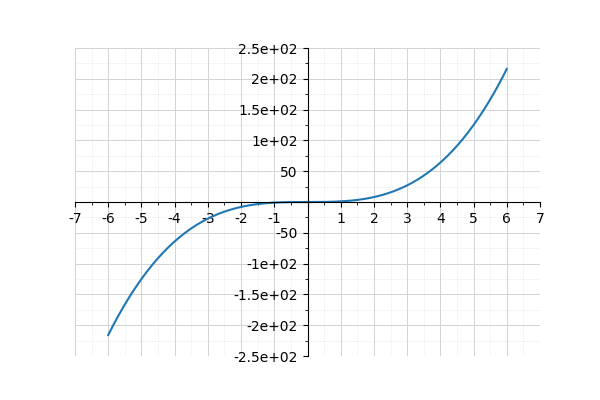
\includegraphics[width=0.7\textwidth]{./img/esponente_dispari.png}
    \caption{Grafico della funzione per $n$ dispari}
    \label{fig:esponente_dispari}
\end{figure}
\FloatBarrier
  
\begin{itemize}
\item La funzione è dispari
\item La funzione è strettamente monotona crescente (quindi è iniettiva $\implies$ invertibile)
\item $\inf_{x \in \mathbb{R}} x^n = -\infty$
\item $\sup_{x \in \mathbb{R}} x^n = +\infty$
\end{itemize}

\subsubsection{Proprietà comuni}
Proprietà valide per entrambi i casi:
\begin{itemize}
\item $x^{n_1} \cdot x^{n_2} = x^{n_1+n_2} \quad \forall x \in \mathbb{R}, \forall n_1, n_2 \in \mathbb{N}$
\item $\frac{x^{n_1}}{x^{n_2}} = x^{n_1-n_2} \quad \text{se } x \neq 0 \text{ e } n_1 \geq n_2$
\item $(x^{n_1})^{n_2} = x^{n_1 \cdot n_2} \quad \forall x \in \mathbb{R}, \forall n_1, n_2 \in \mathbb{N}$
\item $(x \cdot y)^n = x^n \cdot y^n \quad \forall x, y \in \mathbb{R}, \forall n \in \mathbb{N}$
\item $|x^n| = |x|^n \quad \forall x \in \mathbb{R}, \forall n \in \mathbb{N}$
\end{itemize}



\subsubsection{Funzione potenza con esponente negativo}
\defn{Potenza inversa}{
  Si definisce $x^{-n}$ (con $x \neq 0$) come $x^{-n} := \frac{1}{x^n}$
  Poniamo $x^0 = 1$ se $x \neq 0$. A questo punto abbiamo definito la funzione $x^n$ con $n \in \mathbb{Z}$.
}

La funzione potenza con $n$ negativo è definita in:
\begin{itemize}
\item $\mathbb{R} \setminus \{0\}$ per $n$ dispari
\item $(0, +\infty)$ per $n$ pari
\end{itemize}

Grafico della funzione $f(x) = x^n$ con $n$ negativo pari:
\begin{figure}[H]
    \centering
    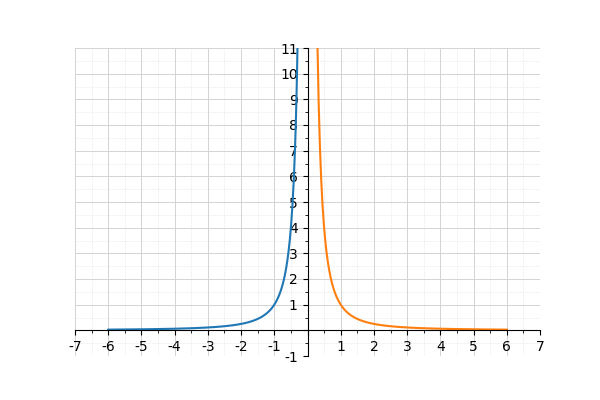
\includegraphics[width=0.7\textwidth]{./img/esponente_neg_pari.png}
    \caption{Grafico della funzione per $n$ negativo pari}
    \label{fig:esponente_neg_pari}
\end{figure}
\FloatBarrier

Grafico della funzione $f(x) = x^n$ con $n$ negativo dispari:
\begin{figure}[H]
    \centering
    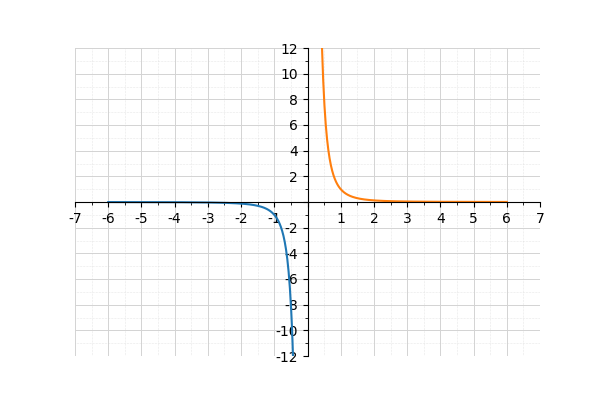
\includegraphics[width=0.7\textwidth]{./img/esponente_neg_dispari.png}
    \caption{Grafico della funzione per $n$ negativo dispari}
    \label{fig:esponente_neg_dispari}
\end{figure}
\FloatBarrier

\subsection{Funzione radice $n$-esima}

\subsubsection{Con esponente dispari}
La funzione potenza con esponente dispari è dotata di inversa: la radice $n$-esima.
$$\sqrt[n]{x}: \mathbb{R} \mapsto \mathbb{R} \quad \text{inversa di } x^n$$

\begin{figure}[H]
    \centering
    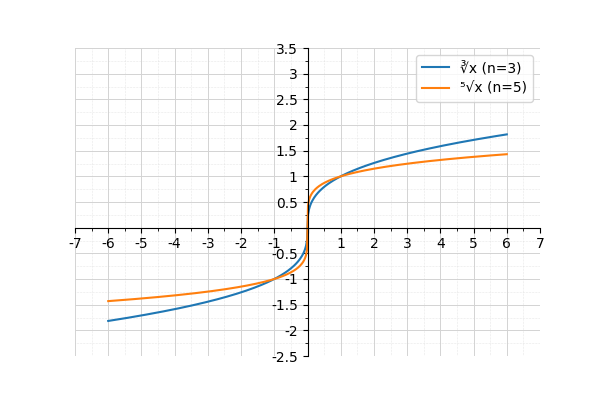
\includegraphics[width=0.7\textwidth]{./img/radice_dispari.png}
    \caption{Grafico della funzione radice $n$-esima con $n$ dispari}
    \label{fig:radice_dispari}
\end{figure}
\FloatBarrier

Proprietà:
\begin{itemize}
\item È strettamente crescente
\item È dispari
\item $\sqrt[n]{x^n} = x \quad \forall x \in \mathbb{R}$
\item $(\sqrt[n]{x})^n = x \quad \forall x \in \mathbb{R}$
\end{itemize}

\subsubsection{Con esponente pari}
La funzione potenza con esponente pari non è globalmente invertibile. Non la possiamo invertire in tutto $\mathbb{R}$; ci serve ridurre il dominio alla parte della funzione strettamente monotona crescente:
$$x^n|_{[0, +\infty[}: [0,+\infty[ \mapsto [0, +\infty[ $$

\begin{figure}[H]
    \centering
    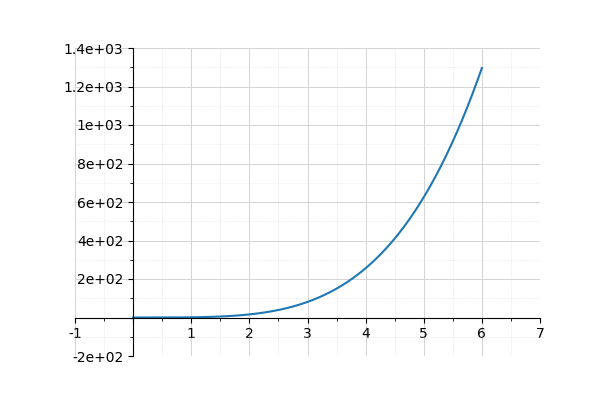
\includegraphics[width=0.7\textwidth]{./img/esponente_pari_ristretta.png}
    \caption{Grafico della restrizione della funzione potenza con $n$ pari}
    \label{fig:potenza_pari_ristretta}
\end{figure}
\FloatBarrier

La funzione inversa della restrizione è la radice $n$-esima:
$$\sqrt[n]{x}: [0, +\infty[ \mapsto [0, +\infty[ $$

\begin{figure}[H]
    \centering
    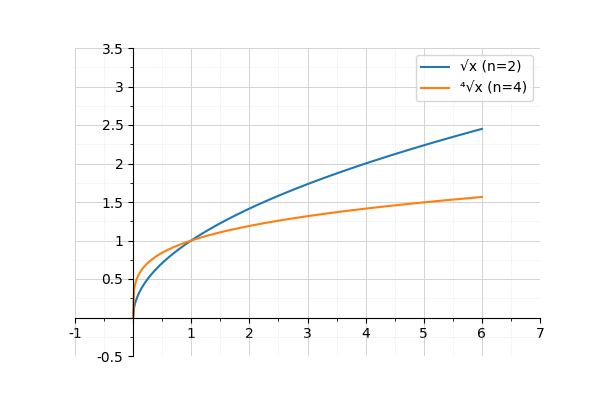
\includegraphics[width=0.7\textwidth]{./img/radice_pari.png}
    \caption{Grafico della funzione radice $n$-esima con $n$ pari}
    \label{fig:radice_pari}
\end{figure}
\FloatBarrier

Come cambiano le relazioni tra la funzione potenza e la sua inversa:
\begin{itemize}
\item $\sqrt[n]{x^n} = |x| \quad \forall x \in \mathbb{R}$
\item $(\sqrt[n]{x})^n = x \quad \forall x \geq 0$
\end{itemize}

\subsubsection{Proprietà comuni}
Proprietà valide per entrambi i casi:
\begin{itemize}
\item $\sqrt[n]{x} \cdot \sqrt[n]{y} = \sqrt[n]{x \cdot y}$ (con $x, y \geq 0$ per $n$ pari)
\item $x < y \implies \sqrt[n]{x} < \sqrt[n]{y}$ (con $x, y \geq 0$ per $n$ pari)
\item $\sqrt[n]{\sqrt[m]{x}} = \sqrt[n \cdot m]{x}$ (con $x \geq 0$ per $n$ o $m$ pari)
\item $\sqrt[n]{x^m} = x^{m/n}$ con $x \geq 0$, $m, n > 0$
\end{itemize}
\end{document}
 
